%!TEX root=../../main.tex
\begin{chapterpage}{Confidence Intervals}
  \chaptertitle{Confidence Intervals}
  \label{ConfidenceIntervals}
  %\chaptersection{variabilityInEstimates}
  \chaptersection{confidenceIntervals}
  \chaptersection{CIwithTDistribution}
  \chaptersection{CIsingleProportion}
  %\chaptersection{hypothesisTesting}
  %\chaptersection{ch4Summary}
  \chaptersection{ch4Exercises}
\end{chapterpage}
\renewcommand{\chapterfolder}{ch_04a_inference_foundations_oi_biostat}

\chapterintro{
A point estimate provides a single plausible value for a parameter. However, a point estimate is rarely perfect; usually there is some error in the estimate. Instead of supplying just a point estimate of a parameter, a next logical step would be to provide a plausible \emph{range of values} for the parameter.

%\subsection{Capturing the population parameter}

A plausible range of values for the population parameter is called a \term{confidence interval}.

Using only a point estimate is like fishing in a murky lake with a spear, and using a confidence interval is like fishing with a net. We can throw a spear where we saw a fish, but we will probably miss. On the other hand, if we toss a net in that area, we have a good chance of catching the fish.

If we report a point estimate, we probably will not hit the exact population parameter. On the other hand, if we report a range of plausible values -- a confidence interval -- we have a good shot at capturing the parameter. 


}


%__________________

%_____________
\section{Confidence intervals}
\label{confidenceIntervals}

\subsection{Interval estimates for a population parameter}

While a point estimate consists of a single value, an interval estimate provides a plausible range of values for a parameter. When estimating a population mean $\mu$, a \term{confidence interval} for $\mu$ has the general form
\[(\overline{x} -m, \ \overline{x} + m) = \overline{x} \pm m, \]
where $m$ is the \term{margin of error}. Intervals that have this form are called \term{two-sided confidence intervals} because they provide both lower and upper bounds, $\overline{x} - m$ and $\overline{x} + m$, respectively. %One-sided sided intervals are discussed in Section~\ref{onesidedCIs}.

The standard error of the sample mean is the standard deviation of its distribution; additionally, the distribution of sample means is nearly normal and centered at $\mu$. Under the normal model, the sample mean $\overline{x}$ will be within 1.96 standard errors (i.e., standard deviations) of the population mean $\mu$ approximately 95\% of the time.\footnote{In other words, the $Z$-score of 1.96 is associated with 2.5\% area to the right (and $Z$ = -1.96 has 2.5\% area to the left); this can be found on normal probability tables or from using statistical software.} Thus, if an interval is constructed that spans 1.96 standard errors from the point estimate in either direction, a data analyst can be 95\% \term{confident} that the interval
\begin{align}
  \overline{x}\ \pm\ 1.96\times \text{SE} 
\label{95PercentCIWhenUsingNormalModel}
\end{align}
contains the population mean. The value 95\% is an approximation, accurate when the sampling distribution for the sample mean is close to a normal distribution. This assumption holds when the sample size is sufficiently large .%(guidelines for `sufficiently large' are given in Section~\ref{ch4Summary}).

\begin{figure}[h]
	\centering
	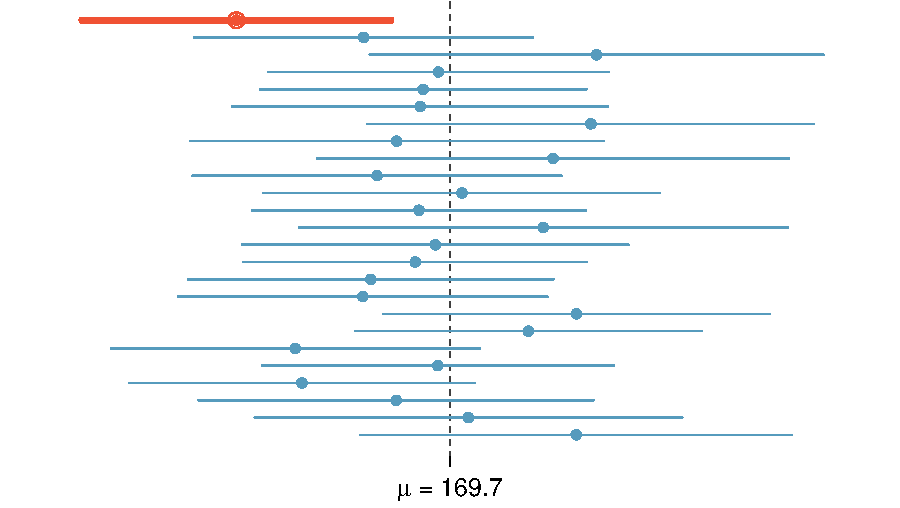
\includegraphics[width=0.66\textwidth]
	{ch_04a_inference_foundations_oi_biostat/figures/95PercentConfidenceInterval/95PercentConfidenceInterval.pdf}
	\caption{Twenty-five samples of size $n=60$ were taken from \data{cdc}. For~each sample, a 95\% confidence interval was calculated for the population average adult weight. Only~1 of these~25 intervals did not contain the population mean, $\mu = 169.7$~lbs.}
	\label{95PercentConfidenceInterval}
\end{figure}

The phrase "95\% confident" has a subtle interpretation: if many samples were drawn from a population, and a confidence interval is calculated from each one using Equation~\ref{95PercentCIWhenUsingNormalModel}, about 95\% of those intervals would contain the population mean $\mu$. Figure~\ref{95PercentConfidenceInterval} illustrates this process with 25 samples taken from \data{cdc}. Of the 25 samples, 24 contain the mean weight in \data{cdc} of 169.7 lbs, while one does not. 

%\textD{\newpage}

Just as with the sampling distribution of the sample mean, the interpretation of a confidence interval relies on the abstract construct of repeated sampling. A data analyst, who can only observe one sample, does not know whether the population mean lies within the single interval calculated. The uncertainty is due to random sampling\textemdash by chance, it is possible to select a sample from the population that has unusually high (or low) values, resulting in a sample mean $\overline{x}$ that is relatively far from $\mu$, and by extension, a confidence interval that does not contain $\mu$. 

\begin{examplewrap}
\begin{nexample}{The sample mean adult weight from the 60 observations in \data{cdc.samp} is $\overline{x}_{\text{weight}} = 173.3$~lbs, and the standard deviation is $s_{\text{weight}} = 49.04$~lbs.  Use Equation~\ref{95PercentCIWhenUsingNormalModel} to calculate an approximate 95\% confidence interval for the average adult weight in the US population.}
  The standard error for the sample mean is  $\text{SE}_{\overline{x}}=\frac{49.04}{\sqrt{60}} = 6.33$~lbs. The 95\% confidence interval is
 \[\overline{x}_{\text{weight}} \pm 1.96 \text{SE}_{\overline{x}} = 173.3 \pm (1.96)(6.33) = (160.89, 185.71)~\text{lbs.} \]
  
  The data support the conclusion that, with 95\% confidence, the average weight of US adults is between approximately 161 and 186~lbs.
  
  Figure~\ref{cdcWeightBigSampDist} visually shows that the sampling distribution is nearly normal. To assess normality of the sampling distribution without repeated sampling, it is necessary to check whether the data are skewed. Although Figure~\ref{cdcWeightHist} shows some skewing, the sample size is large enough that the confidence interval should be reasonably accurate.
\end{nexample}
\end{examplewrap}

\begin{figure}[h]
	\centering
	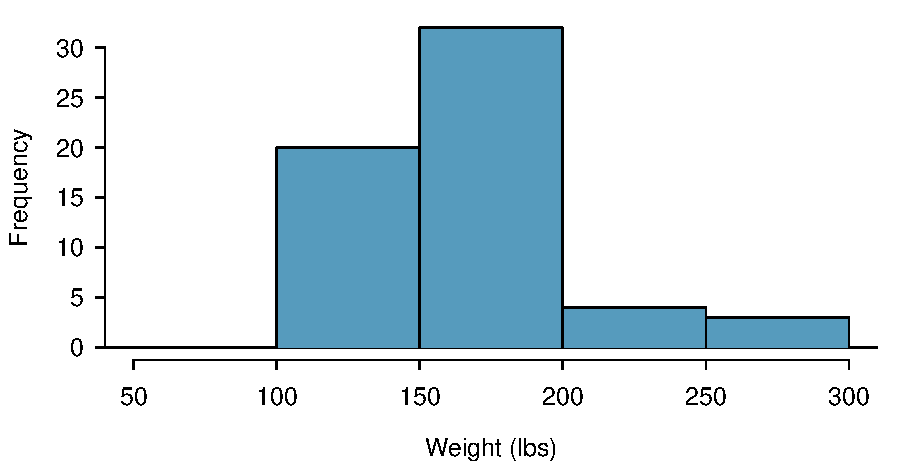
\includegraphics[width=0.65\textwidth]
	{ch_04a_inference_foundations_oi_biostat/figures/cdcWeightHist/cdcWeightHist.pdf}
	\caption{Histogram of \var{weight} in \data{cdc.samp} }
	\label{cdcWeightHist}
\end{figure}

%\textD{\newpage}

\begin{exercisewrap}
\begin{nexercise}\label{95CIExerciseForWeightUSFemales}%
There are 31 females in the sample of 60 US adults, and the average and standard deviation of weight for these individuals are 162.3~lbs and 57.74~lbs, respectively.  A histogram of \var{weight} for the 31 females is shown in Figure~\ref{cdcFemaleWeightHist}.  Calculate an approximate 95\% confidence interval for the average weight of US females.  Is the interval likely to be accurate?\footnotemark{}
\end{nexercise}
\end{exercisewrap}
\footnotetext{Applying Equation~\ref{95PercentCIWhenUsingNormalModel}: $162.3  \pm (1.96)(57.73/\sqrt{31}) \rightarrow (149.85, 174.67)$.  The usual interpretation would be that a data analyst can be about 95\% confident the average weight of US females is between approximately 150 and 175~lbs.  However, the histogram of female weights shows substantial right skewing, and several females with recorded weights larger than 200~lbs. The confidence interval is probably not accurate; a larger sample should be collected in order for the sampling distribution of the mean to be approximately normal.  %Chapter~\ref{inferenceForNumericalData}
  Next section will introduce the $t$-distribution, which is more reliable with small sample sizes than the $z$-distribution.}

\begin{figure}[hht]
   \centering
   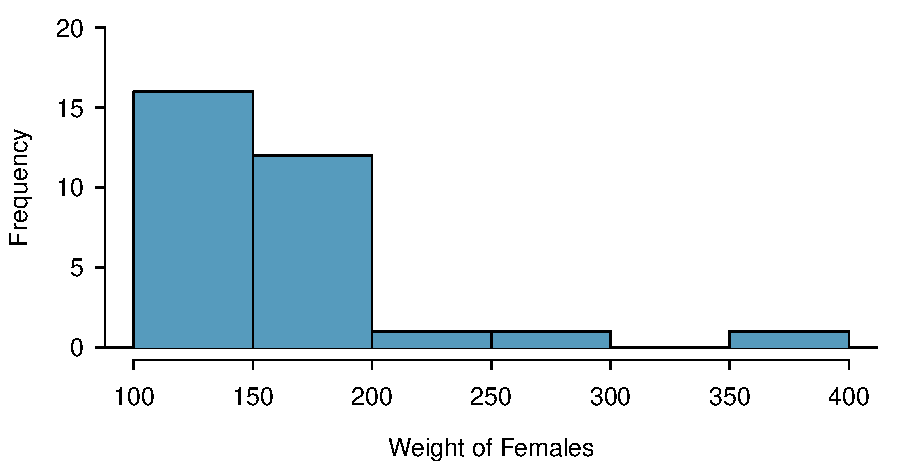
\includegraphics[width=0.7\textwidth]
{ch_04a_inference_foundations_oi_biostat/figures/cdcFemaleWeightHistogram/cdcFemaleWeightHistogram.pdf}
\caption{Histogram of \var{weight} for the 31 females in \data{cdc.samp}.}
\label{cdcFemaleWeightHist}
\end{figure}


\subsection{Changing the confidence level}
\label{changingTheConfidenceLevelSection}

\index{confidence interval!confidence level|(}

Ninety-five percent confidence intervals are the most commonly used interval estimates, but intervals with confidence levels other than 95\% can also be constructed. The general formula for a confidence interval (for the population mean $\mu$) is given by 
\begin{align}
	\overline{x} \pm \ z^{\star} \times \text{SE},
\end{align}
where $z^{\star}$ is chosen according to the confidence level. When calculating a 95\% confidence level, $z^{\star}$ is 1.96, since the area within 1.96 standard deviations of the mean captures 95\% of the distribution.

To construct a 99\% confidence interval, $z^{\star}$ must be chosen such that 99\% of the normal curve is captured between -$z^{\star}$ and $z^{\star}$.

\begin{examplewrap}
\begin{nexample}{Let $Y$ be a normally distributed random variable. Ninety-nine percent of the time, $Y$ will be within how many standard deviations of the mean?}
This is equivalent to the $z$-score with 0.005 area to the right of $z$ and 0.005 to the left of $-z$. In the normal probability table, this is the $z$-value that with 0.005 area to its right and 0.995 area to its left. The closest two values are 2.57 and 2.58; for convenience, round up to 2.58. The unobserved random variable $Y$ will be within 2.58 standard deviations of $\mu$ 99\% of the time, as shown in Figure~\ref{choosingZForCI}.
\end{nexample}
\end{examplewrap}

\begin{figure}[h]
\begin{centering}
	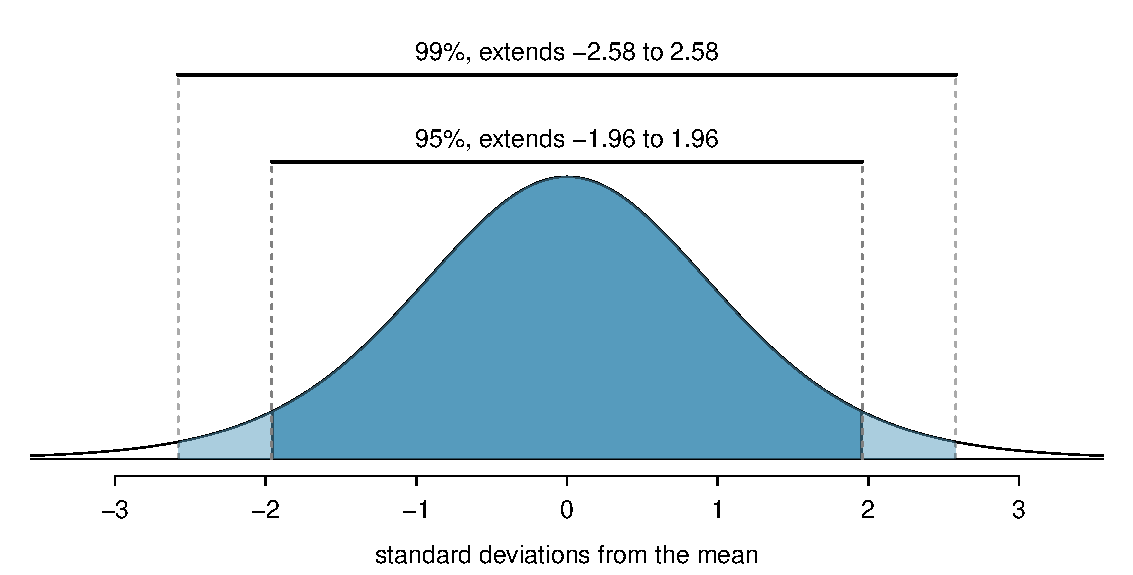
\includegraphics[width=\textwidth]
	{ch_04a_inference_foundations_oi_biostat/figures/choosingZForCI/choosingZForCI.pdf}
	\caption{The area between -$z^{\star}$ and $z^{\star}$ increases as $|z^{\star}|$ becomes larger. If the confidence level is 99\%, $z^{\star}$ is chosen such that 99\% of the normal curve is between -$z^{\star}$ and $z^{\star}$, which corresponds to 0.5\% in the lower tail and 0.5\% in the upper tail: $z^{\star}=2.58$.}
	\label{choosingZForCI}
  \end{centering}
	\index{confidence interval!confidence level|)}
\end{figure}
 
A 99\% confidence interval will have the form 
\begin{align}
	\overline{x} \pm \ 2.58 \times \text{SE},
\end{align}
 and will consequently be wider than a 95\% interval for $\mu$ calculated from the same data, since the margin of error $m$ is larger.


\begin{examplewrap}
\begin{nexample}{Create a 99\% confidence interval for the average adult weight in the US population using the data in \data{cdc.samp}. The point estimate is $\overline{x}_{weight} = 173.3$ and the standard error is $SE_{\overline{x}} = 6.33$.}
Apply the 99\% confidence interval formula: $\overline{x}_{weight}\ \pm\ 2.58 \times  SE_{\overline{x}} \rightarrow (156.97, 189.63)$. A data analyst can be 99\% confident that the average adult weight is between 156.97 and 189.63~lbs.
\end{nexample}
\end{examplewrap}

The 95\% confidence interval for the average adult weight is (160.89, 185.71)~lbs. Increasing the confidence level to 99\% results in the interval (156.97, 189.63) lbs; this wider interval is more likely to contain the population mean $\mu$. However, increasing the confidence level comes at a cost: a wider interval is less informative in providing a precise estimate of the population mean. Consider the extreme: to be "100\% confident" that an interval contains $\mu$, the interval must span all possible values of $\mu$. For example, with 100\% confidence the average weight is between 0 and 1000 lbs; while this interval necessarily contains $\mu$, it has no interpretive value and is completely uninformative.\footnote{Strictly speaking, to be 100\% confident requires an interval spanning all positive numbers; 1000 lbs has been arbitrarily chosen as an upper limit for human weight.} 

Decreasing the confidence level produces a narrower interval; the estimate is more precise, but also more prone to inaccuracy. For example, consider a 50\% confidence interval for average adult weight using \data{cdc.samp}: the $z^{\star}$ value is 0.67, and the confidence interval is (169.06, 177.54)~lbs. This interval provides a more precise estimate of the population average weight $\mu$ than the 99\% or 95\% confidence intervals, but the increased precision comes with less confidence about whether the interval contains $\mu$. In a theoretical setting of repeated sampling, if 100 50\% confidence intervals were computed, only half could be expected to contain $\mu$.

The choice of confidence level is a trade-off between obtaining a precise estimate and calculating an interval that can be reasonably expected to contain the population parameter. In published literature, the most used confidence intervals are the 90\%, 95\%, and 99\%. 

% \subsection{One-sided confidence intervals}
% \label{onesidedCIs}

% One-sided confidence intervals for a population mean provide either a lower bound or an upper bound, but not both.  One-sided confidence intervals have the form
% \[
% (\overline{x} - m, \infty) \text{ or } (-\infty, \overline{x} + m).
% \]

% While the margin of error $m$ for a one-sided interval is still calculated from the standard error of $\overline{x}$ and a $z^\star$ value, the choice of $z^\star$ is a different than for a two-sided interval. For example, the intent of a 95\% one-sided upper confidence interval is to provide an upper bound $m$ such that a data analyst can be 95\% confident that a population mean $\mu$ is less than $\overline{x} + m$. The $z^\star$ value must correspond to the point on the normal distribution that has 0.05 area in the right tail, $z^{\star} = 1.645$.\footnote{Previously, with a two-sided interval, 1.96 was chosen in order to have a total area of 0.05 from both the right and left tails.} A one-sided upper 95\%  confidence interval will have the form
% \begin{align*}
% (-\infty, \overline{x} + 1.645 \times \text{SE}).
% \end{align*}

% \begin{examplewrap}
% \begin{nexample}{Calculate a lower 95\% confidence interval for the population average adult weight in the United States. In the sample of 60 adults in \data{cdc.samp}, the mean and standard error are $\overline{x} = 173.3$ and $SE = 6.33$ days.}
	
% The lower bound is $173.3 - (1.645 \times 6.33) = 163.89$. The lower 95\% interval $(163.89, \infty)$ suggests that one can be 95\% confident that the population average adult weight is at least 163.9~lbs. 
% \end{nexample}
% \end{examplewrap}

% \begin{exercisewrap}
% \begin{nexercise}
% Calculate an upper 99\% confidence interval for the population average adult weight in the United States. The mean and standard error for weight in \data{cdc.samp} are $\overline{x} = 173.3$ and $SE = 6.33$ days.\footnotemark{}
% \end{nexercise}
% \end{exercisewrap}
% \footnotetext{For a one-sided 99\% confidence interval, the $z^\star$ value corresponds to the point with 0.01 area in the right tail, $z^\star = 2.326$. Thus, the upper bound for the interval is $173.3 + (2.326 \times 6.33) = 188.024.$ The upper 99\% interval ($-\infty, 188.024$) suggests that one can be 99\% confident that the population average adult weight is at most 188.0 lbs.}

% %JV: Needs explanation about when to use one-sided interval versus two-sided.


\subsection{Interpreting confidence intervals}
\label{interpretingCIs}

\index{confidence interval!interpretation|(}

The correct interpretation of an XX\% confidence interval is, "We are XX\% confident that the population parameter is between \dots" While it may be tempting to say that a confidence interval captures the population parameter with a certain probability, this is a common error. The confidence level only quantifies how plausible it is that the parameter is within the interval; there is no probability associated with whether a parameter is contained in a specific confidence interval. The confidence coefficient reflects the nature of a procedure that is correct XX\% of the time, given that the assumptions behind the calculations are true.

%\textD{\newpage}

The conditions regarding the validity of the normal approximation can be checked using the numerical and graphical summaries discussed in Chapter 1. However, the condition that data should be from a random sample is sometimes overlooked. If the data are not from a random sample, then the confidence interval no longer has interpretive value, since there is no population mean to which the confidence interval applies. For example, while only simple arithmetic is needed to calculate a confidence interval for BMI from the \data{famuss} dataset in Chapter 1, the participants in the study are almost certainly not a random sample from some population; thus, a confidence interval should not be calculated in this setting.

\begin{examplewrap}
\begin{nexample}{Body mass index (BMI) is one measure of body weight that adjusts for height. The National Health and Nutrition Examination Survey (NHANES) consists of a set of surveys and measurements conducted by the US CDC to assess the health and nutritional status of adults and children in the United States. The dataset \data{nhanes.samp} contains 76 variables and is a random sample of 200 individuals from the measurements collected in the years 2009-2010 and 2012-2013.\footnotemark{} Use \data{nhanes.samp} to calculate a 95\% confidence interval for adult BMI in the US population, and assess whether the data suggest Americans tend to be overweight. \label{exNhanesBmi}}
	
	In the random sample of 200 participants, BMI is available for all 135 of the participants that are 21 years of age or older. As shown in the histogram (Figure~\ref{nhanesAdultBmiHist}), the data are right-skewed, with one large outlier. The outlier corresponds to an implausibly extreme BMI value of 69.0; since it seems likely that the value represents an error from when the data was recorded, this data point is excluded from the following analysis. 
	
	The mean and standard deviation in this sample of 134 are 28.8 and 6.7 $\text{kg}/\text{meter}{^2}$, respectively.  The sample size is large enough to justify using the normal approximation when computing the confidence interval.  The standard error of the mean is $\text{SE} = 6.7/\sqrt{134} = 0.58$, so the 95\% confidence interval is given by 
	\begin{align*}
	\overline{x}_{\text{BMI}} \pm (1.96)(\text{SE}) &= 28.8 \pm (1.96)(0.58) \\
	&= (27.7, 29.9).
	\end{align*}	
	
	Based on this sample, a data analyst can be 95\% confident that the average BMI of US adults is between 27.7 and 29.9 $\text{kg}/\text{m}{^2}$.

The World Health Organization (WHO) and other agencies use BMI to set normative guidelines for body weight. The current guidelines are shown in Figure~\ref{whoBmiGuidelines}. 

%\footnote{\url{http://apps.who.int/bmi/index.jsp?introPage=intro_3.html}}. 

The confidence interval (27.7, 29.9) $\text{kg}/\text{m}{^2}$ certainly suggests that the average BMI in the US population is higher than 21.7, the middle of the range for normal BMIs, and even higher than 24.99, the upper limit of the normal weight category. These data indicate that Americans tend to be overweight. 
\end{nexample}
\end{examplewrap}
\footnotetext{The sample was drawn from a larger sample of 20,293 participants in the \textbf{NHANES} package, available from The Comprehensive R Archive Network (CRAN). The CDC uses a complex sampling design that samples some demographic subgroups with larger probabilities, but \data{nhanes.samp} has been adjusted so that it can be viewed as a random sample of the US population.}

\begin{figure}[h]
		\centering
		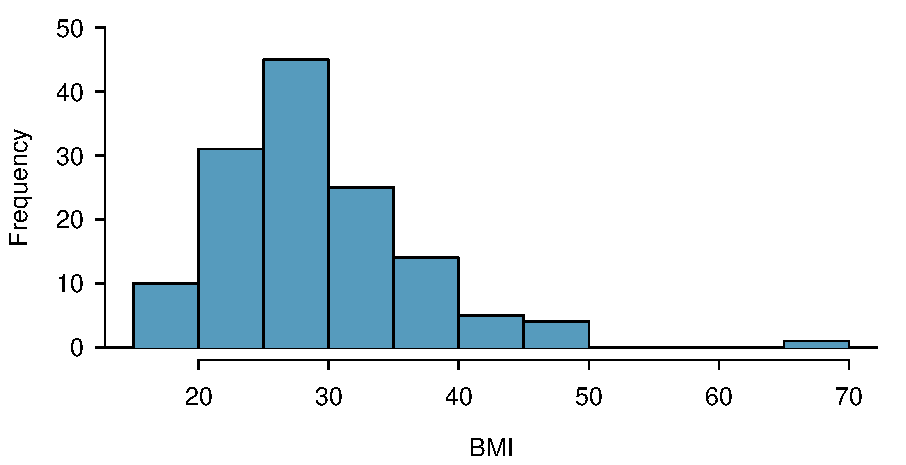
\includegraphics[width=0.8\textwidth]{ch_04a_inference_foundations_oi_biostat/figures/nhanesAdultBmiHist/nhanesAdultBmiHist.pdf}
		\caption{The distribution of \var{BMI} for the 135 adults in \data{nhanes.samp}.}
		\label{nhanesAdultBmiHist}
\end{figure}
	
\begin{figure}[h]
	\begin{center}
		\begin{tabular}{|c|c|}
			\hline 
			Category & BMI range\tabularnewline
			\hline 
			\hline 
			Underweight & $<18.50$\tabularnewline
			\hline 
			Normal (healthy weight) & 18.5-24.99\tabularnewline
			\hline 
			Overweight & $\geq 25$\tabularnewline
			\hline 
			Obese & $\geq30$\tabularnewline
			\hline
		\end{tabular}
		\caption{WHO body weight categories based on BMI.} 
		\label{whoBmiGuidelines}
	\end{center}
\end{figure}



\subsection{Sample size calculation to estimate population mean}
\label{SampleSizeCalculationToEstimate PopulationMean}
Before starting to sample the population to estimate a parameter such as the mean, it is convenient to know how many individuals you need to achieve an accurate estimation with a confidence that the error is lower than a given threshold. Following the previous estimations given in this chapter, the error is the difference between the sample mean (point estimator) and the population mean (true parameter). Confidence interval whose mid point is the sample mean is likely to include the population mean with the given probability $1-\alpha$. Consequently, the error is going to be less than $z_{1-\alpha/2}\sigma/\sqrt{n}$ with that probabiliy.

If the  error of your estimation should be lower than a given threshold or maximum error, then sample size $n$ must be taken large enough such that   $z_{1-\alpha/2}\sigma/\sqrt{n}$ is lower than max. error. Using elementary algebraic reasoning, $n$ should be larger than     $z^2_{1-\alpha/2}\sigma^2/\mbox{max. error}^2 $.

\begin{termBox}{\tBoxTitle{Sample size calculation of $\mu$}
The sample size needed to estimate the population mean, $\mu$ with a maximum error \mbox{max.error} at a confidence $100(1-\alpha)$ and a population variance $\sigma^2$ is 
$n> z^2_{1-\alpha/2}\frac{\sigma^2}{\mbox{max.error}^2} $
.}
%\index{Central Limit Theorem!normal data|)}
\end{termBox}



\begin{example}{
Calculate the sample size you need to estimate the height of male senior in high schools  with a maximum error of 0.1 inches at a confidence of 95\%. We assume that the population standard deviation is $\sigma=3$\,inches   
}
$$n>z^2_{1-\alpha/2}\frac{\sigma^2}{\mbox{max. error}^2}=1.96^2\frac{3^2}{0.1^2}=3457.44	 $$
Therefore, you should take at least 3458 individuals for your sample. 
\end{example}


\index{confidence interval!interpretation|)}
\index{confidence interval|)}



\section[{Single-sample inference with the $t$-distribution}]{Confidence interval  with the $\pmb{\MakeLowercase{t}}$-distribution}
\label{CIwithTDistribution}

\noindent%
The tools studied in the previous section all made use of the $t$-statistic from a sample mean,
\[t = \frac{\overline{x} - \mu}{s/\sqrt{n}},\]
where the parameter $\mu$ is a population mean, $\overline{x}$ and $s$ are the sample mean and standard deviation, and $n$ is the sample size. Tests and confidence intervals were restricted to samples of at least 30 independent observations from a population where there was no evidence of strong skewness. This allowed for the Central Limit Theorem to be applied, justifying use of the normal distribution to calculate probabilities associated with the $t$-statistic. 

In sample sizes smaller than 30, if the data are approximately symmetric and there are no large outliers, the $t$-statistic has what is called a $t$-distribution. When the normal distribution is used as the sampling distribution of the $t$-statistic, $s$ is essentially being treated as a good replacement for the unknown population standard deviation $\sigma$. However, the sample standard deviation $s$, as an estimate of $\sigma$, has its own inherent variability like $\overline{x}$. The $t$ density function adjusts for the variability in $s$ by having more probability in the left and right tails than the normal distribution.

\subsection{The $\pmb{\MakeLowercase{t}}$-distribution}
\label{introducingTheTDistribution}

\index{t-distribution|(}
\index{distribution!$t$|(}

Figure~\ref{tDistCompareToNormalDist} shows a $t$-distribution and normal distribution. Like the standard normal distribution, the $t$-distribution is unimodal and symmetric about zero.  However, the tails of a $t$-distribution are thicker than for the normal, so observations are more likely to fall beyond two standard deviations from the mean than under the normal distribution.\footnote{The standard deviation of the $t$-distribution is actually a little more than 1. However, it is useful to think of the $t$-distribution as having a standard deviation of 1 in the context of using it to conduct inference.} While the estimate of the standard error will be less accurate with smaller sample sizes, the thick tails of the $t$-distribution correct for the variability in $s$.

\begin{figure}[h]
\centering
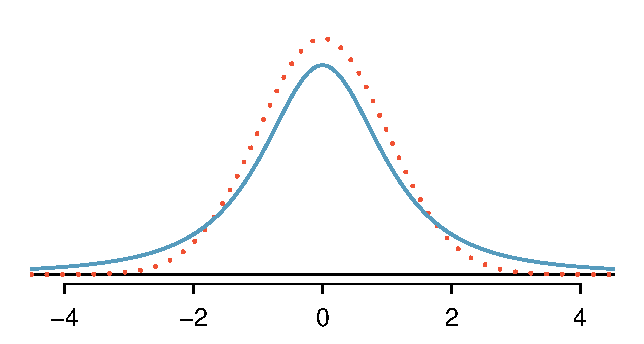
\includegraphics[width=0.5\textwidth]{ch_06a_inference_for_means_oi_biostat/figures/tDistCompareToNormalDist/tDistCompareToNormalDist}
\caption{Comparison of a $t$-distribution (solid line) and a normal distribution (dotted line).}
\label{tDistCompareToNormalDist}
\end{figure}

The $t$-distribution can be described as a family of symmetric distributions with a single parameter: degrees of freedom, which equals $n - 1$. Several $t$-distributions are shown in Figure~\ref{tDistConvergeToNormalDist}. When there are more degrees of freedom, the $t$-distribution looks very much like the standard normal distribution. With degrees of freedom of 30 or more, the $t$-distribution is nearly indistinguishable from the normal distribution. Since the $t$-statistics in Chapter~\ref{foundationsForInference} were associated with sample sizes of at least 30, the degrees of freedom for the corresponding $t$-distributions were large enough to justify use of the normal distribution to calculate probabilities.

%\textD{\newpage}

\begin{figure}
\centering
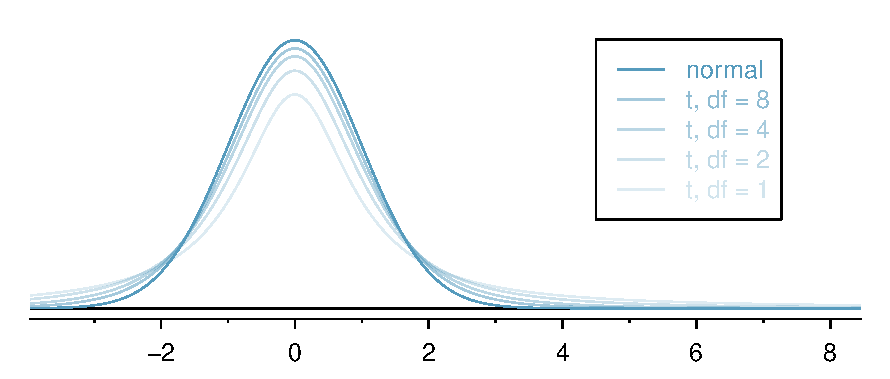
\includegraphics[width=0.75\textwidth]{ch_06a_inference_for_means_oi_biostat/figures/tDistConvergeToNormalDist/tDistConvergeToNormalDist}
\caption{The larger the degrees of freedom, the more closely the $t$-distribution resembles the standard normal model.}
\label{tDistConvergeToNormalDist}
\end{figure}

\begin{onebox}{Degrees of freedom (df)}
The degrees of freedom characterize the shape of the $t$-distribution. The larger the degrees of freedom, the more closely the distribution approximates the normal model.
\end{onebox}

Probabilities for the $t$-distribution can be calculated either by using distribution tables or using statistical software. The use of software has become the preferred method because it is more accurate, allows for complete flexibility in the choice of $t$-values on the horizontal axis, and is not limited to a small range of degrees of freedom. The remainder of this section illustrates the use of a \term{t-table}, partially shown in Figure~\ref{tTableSample}, in place of the normal probability table. A larger $t$-table is in Appendix~\ref{tDistributionTable} on page~\pageref{tDistributionTable}.  The \textsf{R} labs illustrate the use of software to calculate probabilities for the $t$-distribution.  Readers intending to use software can skip to the next section.


\begin{figure}[hht]
\centering
\begin{tabular}{r | rrr rr}
  df/p & \hspace{1.5mm}  0.9 & \hspace{1.5mm} 0.95 & \hspace{1.5mm} 0.975 & \hspace{1.5mm} 0.99 & \hspace{1.5mm} 0.995  \\
%one tail & \hspace{1.5mm}  0.100 & \hspace{1.5mm} 0.050 & \hspace{1.5mm} 0.025 & \hspace{1.5mm} 0.010 & \hspace{1.5mm} 0.005  \\
%two tails & 0.200 & 0.100 & 0.050 & 0.020 & 0.010 \\
\hline
{$df$} \hfill 1  &  {\normalsize  3.08} & {\normalsize  6.31} & {\normalsize 12.71} & {\normalsize 31.82} & {\normalsize 63.66}  \\ 
2  &  {\normalsize  1.89} & {\normalsize  2.92} & {\normalsize  4.30} & {\normalsize  6.96} & {\normalsize  9.92}  \\ 
3  &  {\normalsize  1.64} & {\normalsize  2.35} & {\normalsize  3.18} & {\normalsize  4.54} & {\normalsize  5.84}  \\ 
$\vdots$ & $\vdots$ &$\vdots$ &$\vdots$ &$\vdots$ & \\
17  &  {\normalsize  1.33} & {\normalsize  1.74} & {\normalsize  2.11} & {\normalsize  2.57} & {\normalsize  2.90}  \\ 
\highlightO{18}  &  \highlightO{\normalsize  1.33} & \highlightO{\normalsize  1.73} & \highlightO{\normalsize  2.10} & \highlightO{\normalsize  2.55} & \highlightO{\normalsize  2.88}  \\ 
19  &  {\normalsize  1.33} & {\normalsize  1.73} & {\normalsize  2.09} & {\normalsize  2.54} & {\normalsize  2.86}  \\ 
20  &  {\normalsize  1.33} & {\normalsize  1.72} & {\normalsize  2.09} & {\normalsize  2.53} & {\normalsize  2.85}  \\ 
$\vdots$ & $\vdots$ &$\vdots$ &$\vdots$ &$\vdots$ & \\
400  &  {\normalsize  1.28} & {\normalsize  1.65} & {\normalsize  1.97} & {\normalsize  2.34} & {\normalsize  2.59}  \\ 
500  &  {\normalsize  1.28} & {\normalsize  1.65} & {\normalsize  1.96} & {\normalsize  2.33} & {\normalsize  2.59}  \\ 
$\infty$  &  {\normalsize  1.28} & {\normalsize  1.64} & {\normalsize  1.96} & {\normalsize  2.33} & {\normalsize  2.58}  \\ 
\end{tabular}
\caption{An abbreviated look at the $t$-table. Each row represents a different $t$-distribution. The columns describe the cutoffs for specific tail areas. The row with $df=18$ has been \highlightO{highlighted}.}
\label{tTableSample}
\end{figure}

Each row in the $t$-table represents a $t$-distribution with different degrees of freedom. The columns correspond to percentiles. For instance, for a $t$-distribution with $df=18$, row 18 is used (highlighted in Figure~\ref{tTableSample}). The value in this row that identifies the cutoff for an upper tail of 5\% is found in the column where \emph{one tail} is 0.950. This cutoff is 1.73. The cutoff for the lower 5\% is -1.73; just like the normal distribution, all $t$-distributions are symmetric. 

%\textD{\newpage}

\begin{examplewrap}
  \begin{nexample}{What proportion of the $t$-distribution with 18 degrees of freedom falls below -2.10?}

    Just like a normal probability problem, we first draw the picture in Figure~\ref{tDistDF18LeftTail2Point10} and shade the area below -2.10. The area on the left of -2.10 is the same area that on the right of 2.10. In the $t$ distribution are the percentiles corresponding to positive values. To find this area, we identify the appropriate row: $df=18$. Then we identify the column containing the absolute value of -2.10; a very similar value  is at the last but two column and the corresponding quantile os 0.975. Hence, on the left of 2.10 the area is 0.975 and, consequently, the area on the right is 0.025. About 2.5\% of the distribution falls below -2.10. In the next example we encounter a case where the exact $t$ value is not listed in the table.

    
\end{nexample}
\end{examplewrap}

\begin{figure}[h]
\centering
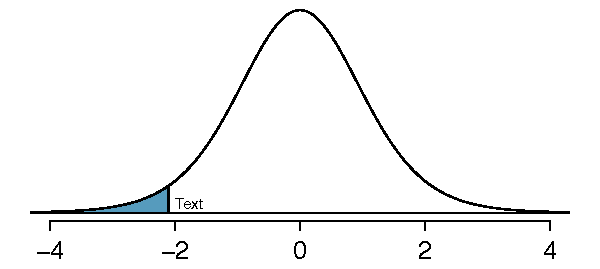
\includegraphics[width=0.55\textwidth]{ch_06a_inference_for_means_oi_biostat/figures/tDistDF18LeftTail2Point10/tDistDF18LeftTail2Point10}
\caption{The $t$-distribution with 18 degrees of freedom. The area below -2.10 has been shaded.}
\label{tDistDF18LeftTail2Point10}
\end{figure}

\begin{examplewrap}
  \begin{nexample}{A $t$-distribution with 20 degrees of freedom is shown in the left panel of Figure~\ref{tDistDF20RightTail1Point65}. Estimate the proportion of the distribution falling above 1.65 and below -1.65.}
We identify the row in the $t$ table using the degrees of freedom: $df=20$. Then we look for 1.65; it is not listed. It falls between the  columns corresponding to 0.900 and 0.9500. Since these values bound 1.65, their tail areas will bound the tail area corresponding to 1.65. These are the values of area on the left but the question is about values on the right. So, the area on the right is between  0.050 and 0.10, and we conclude that between 5\% and 10\% of the distribution is more than 1.65 standard deviations above the mean. If we like, we can identify the precise area using statistical software: 0.0573.

%Identify the row in the $t$-table using the degrees of freedom: $df-20$. Then, look for 1.65; the value is not listed, and falls between the first and second columns. Since these values bound 1.65, their tail areas will bound the tail area corresponding to 1.65. The two tail area of the first and second columns is between 0.100 and 0.200. Thus, between 10\% and 20\% of the distribution is more than 1.65 standard deviations from the mean. The precise area can be calculated using statistical software: 0.1146.
\end{nexample}
\end{examplewrap}

\begin{figure}[h]
	\centering
	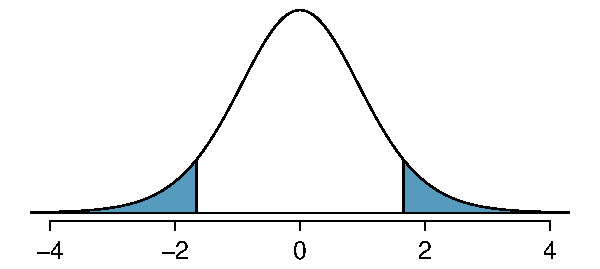
\includegraphics[width=0.55\textwidth]{ch_06a_inference_for_means_oi_biostat/figures/tDistDF20RightTail1Point65/tDistDF20RightTail1Point65}
	\caption{The $t$-distribution with 20 degrees of freedom, with the area further than 1.65 away from 0 shaded.}
	\label{tDistDF20RightTail1Point65}
\end{figure}

\index{t-distribution|)}
\index{distribution!$t$|)}


%\textD{\newpage}


\subsection{Using the $\pmb{\MakeLowercase{t}}$-distribution for tests and confidence intervals for a population mean}

\label{oneSampleTConfidenceIntervalsTests}

\index{t-test!one-sample|(}

Section~\ref{confidenceIntervals} provided formulas for  confidence intervals for population means in random samples large enough for the $t$-statistic to have a nearly normal distribution.  In samples smaller than 30 from approximately symmetric distributions without large outliers, the $t$-statistic has a $t$-distribution with degrees of freedom equal to $n - 1$. Just like inference in larger samples, inference using the $t$-distribution also requires that the observations in the sample be independent.  Random samples from very large populations always produce independent observations;  in smaller populations, observations will be approximately independent as long as the size of the sample is no larger than 10\% of the population.

In summary, to proceed with the $t$ distribution for inference about a single mean, we must check two conditions.
\begin{description}
\item[Independence of observations.] We verify this condition just as we did before. We collect a simple random sample from less than 10\% of the population, or if it was an experiment or random process, we carefully check to the best of our abilities that the observations were independent.
\item[Observations come from a nearly normal distribution.] This second condition is difficult to verify with small data sets. We often (i) take a look at a plot of the data for obvious departures from the normal model, and (ii) consider whether any previous experiences alert us that the data may not be nearly normal.
\end{description}

Formulas for tests and intervals using the $t-$distribution are very similar to those using the normal distribution.  For a sample of size $n$ with sample mean $\overline{x}$ and standard deviation $s$, two-sided confidence intervals with confidence coefficient $100(1 - \alpha)$\% have the form
\[
    \overline{x} \pm t_{\text{df}}^{\star} \times \text{SE},
\]
where SE is the standard error of the sample mean ($s/\sqrt{n}$) and $t_{\text{df}}^{\star}$ is the point on a $t$-distribution with $n-1$ degrees of freedom and area $(1 - \alpha/2)$ to its left.

A one-sided interval with the same confidence coefficient will have the form  
\begin{align*}
    \overline{x} &+ t_{\text{df}}^{\star} \times \text{SE} \text{   (one-sided upper confidence interval)}, \text{  or} \\
    \overline{x} &- t_{\text{df}}^{\star} \times \text{SE} \text{   (one-sided lower confidence interval)},
\end{align*}
except that in this case $t_{\text{df}}^{\star}$ is the point on a $t$-distribution with $n-1$ degrees of freedom and  area $(1 - \alpha)$ to its left.

With the ability to conveniently calculate $t^\star$ for any sample size or associated $\alpha$ via computing software, the $t$-distribution can be used by default over the normal distribution. The rule of thumb that $n > 30$ qualifies as a large enough sample size to use the normal distribution dates back to when it was necessary to rely on distribution tables.

\index{data!dolphins and mercury|(}
\begin{examplewrap}
\begin{nexample}{Dolphins are at the top of the oceanic food chain; as a consequence, dangerous substances such as mercury tend to be present in their organs and muscles at high concentrations. In areas where dolphins are regularly consumed, it is important to monitor dolphin mercury levels. This example uses data from a random sample of 19 Risso's dolphins from the Taiji area in Japan.\footnotemark{} Calculate the 95\% confidence interval for average mercury content in Risso's dolphins from the Taiji area using the data in Figure~\ref{summaryStatsOfHgInMuscleOfRissosDolphins}.}

The observations are a simple random sample consisting of less than 10\% of the population, so independence of the observations is reasonable. The summary statistics in Figure~\ref{summaryStatsOfHgInMuscleOfRissosDolphins} do not suggest any skew or outliers; all observations are within 2.5 standard deviations of the mean. Based on this evidence, the approximate normality assumption seems reasonable.

Use the $t$-distribution to calculate the confidence interval:
\begin{align*}
\overline{x} \pm  t^{\star}_{\text{df}} \times \text{SE} &= \overline{x}  \pm  t^{\star}_{18}  \times s/\sqrt{n} \\
&= 4.4 \pm  2.10 \times 2.3/\sqrt{19} \\
&= (3.29, 5.51)\,\, \mu\text{g/wet g}.
\end{align*}

The $t^{\star}$ point can be read from the $t$-table on page~\pageref{tTableSample}, in the column with area totaling 0.05 in the two tails (third column) and the row with 18 degrees of freedom. Based on these data, one can be 95\% confident the average mercury content of muscles in Risso's dolphins is between 3.29 and 5.51 $\mu$g/wet gram.

Alternatively, the $t^\star$ point can be calculated in \textsf{R} with the function \texttt{qt}, which returns a value of 2.1009.
\end{nexample}
\end{examplewrap}
\footnotetext{Taiji is a significant source of dolphin and whale meat in Japan. Thousands of dolphins pass through the Taiji area annually; assume that these 19 dolphins represent a simple random sample. Data reference: Endo T and Haraguchi K. 2009. High mercury levels in hair samples from residents of Taiji, a Japanese whaling town. Marine Pollution Bulletin 60(5):743-747.}

\begin{figure}[h]
	\centering
	\begin{tabular}{ccc cc}
		\hline
		$n$ & $\overline{x}$ & $s$ & minimum & maximum \\
		19   & 4.4	  & 2.3  & 1.7	       & 9.2 \\
		\hline
	\end{tabular}
	\caption{Summary of mercury content in the muscle of 19 Risso's dolphins from the Taiji area. Measurements are in $\mu$g/wet g (micrograms of mercury per wet gram of muscle).}
	\label{summaryStatsOfHgInMuscleOfRissosDolphins}
\end{figure}		
		
\index{data!dolphins and mercury|)}

%\textD{\newpage}

\begin{exercisewrap}
\begin{nexercise}\label{croakerWhiteFishPacificExerConditions}%
\index{data!white fish and mercury|(}%
The FDA's webpage provides some data on mercury content of various fish species.\footnotemark{} From a sample of 15 white croaker (Pacific), a sample mean and standard deviation were computed as 0.287 and 0.069 ppm (parts per million), respectively. The 15 observations ranged from 0.18 to 0.41 ppm. Assume that these observations are independent. Based on summary statistics, does the normality assumption seem reasonable? If so, calculate a 90\% confidence interval for the average mercury content of white croaker (Pacific).\footnotemark{}
\end{nexercise}
\end{exercisewrap}
\addtocounter{footnote}{-1}%
\footnotetext{\oiRedirect{textbook-fda_mercury_in_fish_2010}{www.fda.gov/food/foodborneillnesscontaminants/metals/ucm115644.htm}}%
\addtocounter{footnote}{1}%
\footnotetext{There are no obvious outliers; all observations are within 2 standard deviations of the mean. If there is skew, it is not evident. There are no red flags for the normal model based on this (limited) information. $\overline{x} \ \pm\ t^{\star}_{14} \times SE \ \to\  0.287 \ \pm\  1.76\times 0.0178\ \to\ (0.256, 0.318)$. We are 90\% confident that the average mercury content of croaker white fish (Pacific) is between 0.256 and 0.318 ppm.}


%__________

%%%% ANYADIDO: CAP. 8

\section{Confidence interval for a single proportion}
\label{CIsingleProportion}

Advanced melanoma is an aggressive form of skin cancer that until recently was almost uniformly fatal.  In rare instances, a patient's melanoma stopped progressing or disappeared altogether when the patient's immune system successfully mounted a response to the cancer. Those observations led to research into therapies that might trigger an immune response in cancer.  Some of the most notable successes have been in melanoma, particularly with two new therapies, nivolumab and ipilimumab\footnote{The -mab suffix in these therapies stands for monoclonal antibody, a therapeutic agent made by identical immune cells that are all clones of a unique parent cell from a patient.}.

A 2013 report in the New England Journal of Medicine by Wolchok et al. reported the results of a study in which patients were treated with both nivolumab and ipilimumab.\footnote{N Engl J Med 2013;369:122-33. DOI: 10.1056/NEJMoa1302369}   Fifty-three patients were given the new regimens concurrently, and the response to therapy could be evaluated in 52 of the 53.  Of the 52 evaluable patients, 21 (40\%) experienced a response according to commonly accepted criteria.  In previous studies, the proportion of patients responding to one of these agents was 30\% or less.  How might one compare the new data to past results?

The data from this study are binomial data, with success defined as a response to therapy. Suppose the number of patients who respond in a study like this is represented by the random variable $X$, where $X$ is binomial with parameters $n$ (the number of trials, where each trial is represented by a patient) and $p$ (the unknown population proportion of response). From formulas discussed in Chapter~\ref{modeling}, the mean of $X$ is $np$ and the standard deviation of $X$ is $\sqrt{np(1-p)}$.

Inference about $p$ is based on the sample proportion $\hat{p}$, where $\hat{p} = X/n$. In this case, $\hat{p} = 21/52 = 0.404$. If the sample proportion is nearly normally distributed, the normal approximation to the binomial distribution can be used to conduct inference; this method is commonly used.  %When $X$ does not have an approximately normal distribution, exact inference can  based on the binomial distribution for $X$.  Both the normal approximation and exact methods are covered in this chapter.

\subsection{Inference using the normal approximation}

A \term{sample proportion} can be described as a sample mean. If each success in the melanoma data  is represented as a \texttt{1} and each failure as a \texttt{0}, then the sample proportion is the mean of the 52 numerical outcomes:
\begin{eqnarray*}
\hat{p} = \frac{\ 0 + 1 + 1 + \cdots + 0\ }{52} = 0.404.
\end{eqnarray*}
The distribution of $\hat{p}$ is nearly normal when the distribution of successes and failures is not too strongly skewed.

\textD{\newpage}

\index{sampling distribution!sample proportion}

\begin{onebox}{Conditions for the sampling distribution of $\pmb{\hat{\MakeLowercase{p}}}$ being nearly normal}
The sampling distribution for $\hat{p}$, calculated from a sample of size $n$ from a population with a success proportion $p$, is nearly normal when
\begin{enumerate}
\item the sample observations are independent and
\item at least 10 successes and 10 failures are expected in the sample, i.e. $np\geq10$ and $n(1-p)\geq10$. This is called the \term{success-failure condition}.
\end{enumerate}
If these conditions are met, then the sampling distribution of $\hat{p}$ is approximately normal with mean $p$ and standard error
\index{standard error (SE)!single proportion}
\begin{eqnarray}
SE_{\hat{p}} = \sqrt{\frac{p(1-p)}{n}}.
\label{seOfPHat}
\end{eqnarray}
\end{onebox}%
\marginpar[\raggedright\vspace{-53mm}

$\hat{p}$\vspace{0mm}\\\footnotesize sample\\proportion\vspace{3mm}\\\normalsize$p$\vspace{0mm}\\\footnotesize population\\proportion]{\raggedright\vspace{-53mm}

$\hat{p}$\vspace{0mm}\\\footnotesize sample\\proportion\vspace{3mm}\\\normalsize$p$\vspace{0mm}\\\footnotesize population\\proportion}

When conducting inference, the population proportion $p$ is unknown. Thus, to construct a confidence interval, the sample proportion $\hat{p}$ can be substituted for $p$ to check the success-failure condition and compute the standard error. %In a hypothesis test, $p_0$ is substituted for $p$.

\subsubsection{Confidence intervals for a proportion}
\label{confIntForPropSection}

\index{point estimate!single proportion}
\index{confidence interval!single proportion}

When using the normal approximation to the sampling distribution of $\hat{p}$, a confidence interval for a proportion has the same structure as a confidence interval for a mean; it is centered at the point estimate, with a margin of error calculated from the standard error and appropriate $z^{\star}$ value.  The formula for a 95\% confidence interval is
\[
  \hat{p} \pm 1.96 \sqrt{\frac{\hat{p}(1-\hat{p})}{n}}.
\]

\begin{examplewrap}
\begin{nexample}{Using the normal approximation, construct an approximate 95\% confidence interval for the response probability for patients with advanced melanoma who were administered the combination of nivolumab and ipilimumab.}

The independence and success-failure assumptions should be checked first.  Since the outcome of one patient is unlikely to influence that of other patients, the observations are independent.  The success-failure condition is satisfied since $n\hat{p} = (52)(.404) = 21  > 10$ and $n\hat{p}(1 - \hat{p}) = (52)(.596) = 31  > 10$.

The point estimate for the response probability, based on a sample of size $n = 52$, is $\hat{p} = 0.404$. For a 95\% confidence interval, $z^{\star} = 1.96$. The standard error is estimated as: $\sqrt{\frac{\ \hat{p}(1-\hat{p})\ }{n}} = \sqrt{\frac{(0.404)(1-0.404)}{52}} = 0.068$.  The confidence interval is
\[0.404 \pm 1.96 (0.068) \rightarrow (0.27, 0.54) \]
The approximate 95\% confidence interval for $p$, the population response probability of melanoma patients to the combination of these new drugs, is (0.27, 0.54) or (27\%, 54\%).  
\end{nexample}
\end{examplewrap}

%\textD{\newpage}

\begin{exercisewrap}
\begin{nexercise}
In New York City on October 23rd, 2014, a doctor who had recently been treating Ebola patients in Guinea went to the hospital with a slight fever and was subsequently diagnosed with Ebola. Soon after, a survey conducted by the Marist Poll, an organization with a carefully designed methodology for drawing random samples from identified populations, found that 82\% of New Yorkers favored a "mandatory 21-day quarantine for anyone who has come in contact with an Ebola patient."\footnotemark{} a) Verify that the sampling distribution of $\hat{p}$ is nearly normal. b) Construct a 95\% confidence interval for $p$, the proportion of New York adults who supported a quarantine for anyone who has come into contact with an Ebola patient.\footnotemark{}
\end{nexercise}
\end{exercisewrap}
\addtocounter{footnote}{-1}%
\footnotetext{\oiRedirect{textbook-maristpoll_ebola_201410}{Poll ID NY141026 on maristpoll.marist.edu}.}%
\addtocounter{footnote}{1}%
\footnotetext{a) The poll is based on a simple random sample and consists of fewer than 10\% of the adult population of New York, which makes independence a reasonable assumption. The success-failure condition is satisfied since, $1042(0.82) > 5$ and $1042(1-0.82) > 5$. b) $0.82 \pm 1.96\sqrt{\frac{0.82(1-0.82)}{1042}} \rightarrow (0.796, 0.844)$.}

Did the participants in the melanoma trial constitute a random sample?  Patients who participate in clinical trials are unlikely to be a random sample of patients with the disease under study since the patients or their physicians must be aware of the trial, and patients must be well enough to travel to a major medical center and be willing to receive an experimental therapy that may have serious side effects.  

Investigators in the melanoma trial were aware that the observed proportion of patients responding in a clinical trial may be different than the hypothetical response probability in the population of patients with advanced melanoma. Study teams try to minimize these systematic differences by following strict specifications for deciding whether patients are eligible for a study. However, there is no guarantee that the results observed in a sample will be replicated in the general population.

Small, initial studies in which there is no control group, like the one described here, are early steps in exploring the value of a new therapy and are used to justify further study of a treatment when the results are substantially different than expected.  The largest observed response rate in previous trials of 30\% was close to the lower bound of the confidence interval from the study (27\%, 54\%), so the results were considered adequate justification for continued research on this treatment.
\subsection{Sample size calculation of population proportion}
\label{SampleSizeCalculationofPopulationProportion}

Before sampling your population to estimate a proportion is convenient to now the sample size you will need. The theoretical reasoning  to get the formula is similar to the seen in the section~\ref{SampleSizeCalculationToEstimate PopulationMean}. However, for the standard error of the proportion is depending on the population proportion, which is the unknown value to estimate.  To prevent this problem, a pre-estimated value $p_0$ of the population proportion is used. 

\begin{termBox}{\tBoxTitle[]{Formula to estimate the sample size}  \vspace{-1mm}
The sample size to estimate the population proportion with a maximum error, $\mbox{max.error}$, at a confidence $100(1-\alpha)$\% with a previously estimated value $p_0$. 
$$n> \frac{z_{1-\alpha/2}^2p_0(1-p_0)}{\mbox{max.error}^2}$$ 
  }
\end{termBox}
\begin{example}{     What is the number of dogs we we need to estimate the proportion
    of stray dogs
    vaccinated of leptospirosis with a confidence of 95\% of the
    (absolute) error
    being less than 5\%? From the data in a vet clinic, we have
    a rough idea that they are going to be around 65\% with a 
    confidence of 95\% }
  Our confidence is 95\%, so  $\alpha=0.05$ and  $1-\alpha/2=0.975$. The z-score to use is  $z_{0.975}=1.96$ and applying the formula with $p_0=0.65$ 
    $$ n> \frac{1.96^2 \cdot 0.65 \cdot 0.35}{0.05^2}=349.5856$$
    So, we need at least 350 dogs.
\end{example}

In some settings a preliminary estimate for $p$ can be used to calculate $n$.  When no estimate is available, calculus can be used to show that $p(1 - p)$ has its largest value when $p = 0.50$, and that conservative value for $p$ is often used to ensure that $n$ is sufficiently large regardless of the value of the unknown population proportion $p$.  In  that case, $n$ satisfies
\begin{align*}
  n \geq \frac{(z_{1-\alpha/2})^2(0.50)(1-0.50)}{m^2} = \frac{(z_{1-\alpha/2})^2}{4m^2}.
\end{align*}

%\textD{\newpage}

\begin{examplewrap}
\begin{nexample}{Donor organs for organ transplant are scarce. Studies are conducted to explore whether the population of eligible organs can be expanded. Suppose a research team is studying the possibility of transplanting lungs from hepatitis C positive individuals; recipients can be treated with one of the new drugs that cures hepatitis C. Preliminary studies in organ transplant are often designed to estimate the probability of a successful organ graft 6 months after the transplant.  How large should a study be so that the 95\% confidence interval for the probability of a successful graft at 6 months is no wider than 20\%?}

A confidence interval no wider than 20\% has a margin of error of 10\%, or 0.10.  Using the conservative value p = 0.50,
\[n = \frac{(1.96)^2}{(4)(0.10^2)} =  96.04.\]
Sample sizes are always rounded up, so the study should have 97 patients.  

Since the study will likely yield a value $\hat{p}$ different from 0.50, the final margin of error will be smaller than $\pm 0.10$.
\end{nexample}
\end{examplewrap}

When the confidence coefficient is 95\%, 1.96 can replaced by 2 and the sample size formula reduces to 
\begin{align*}
  n = 1/m^2.
\end{align*}
This remarkably simple formula is often used by practitioners for a quick estimate of sample size.

\index{sample size!estimating a proportion|)}

\index{data!Congress approval rating|(}

\begin{exercisewrap}
\begin{nexercise}
A 2015 estimate of Congress' approval rating was 19\%.\footnotemark{} Using this estimate, how large should an additional survey be to produce a margin of error of 0.04 with 95\% confidence?\footnotemark{}
\end{nexercise}
\end{exercisewrap}
\addtocounter{footnote}{-1}%
\footnotetext{\oiRedirect{textbook-congress_at_19_in_May2015}{www.gallup.com/poll/183128/five-months-gop-congress-approval-remains-low.aspx}}%
\addtocounter{footnote}{1}%
\footnotetext{Apply the formula \\
\begin{align*}
1.96\times \sqrt{\frac{p(1-p)}{n}} \approx
1.96\times \sqrt{\frac{0.19(1-0.19)}{n}} &\leq 0.04 \qquad\to\qquad n \geq 369.5.
\end{align*}
A sample size of 370 or more would be reasonable.}

\index{data!Congress approval rating|)}
\index{margin of error|)}

Sample size calculation is an essential step for a experimental design not only for estimation, but also for hypothesis testings, which are going to be studied during next units. However, these sample calculate are out of the scope of this introductory courses and we are not going to provide more details in  units to come. 


